\documentclass{article}

\textwidth=6.5in
\textheight=8.5in
\voffset=-54pt
\oddsidemargin=0in
\evensidemargin=0in
\setlength{\parskip}{8pt}
\setlength{\parindent}{0pt}

\usepackage{workbook}

\usepackage[]{handout}

\begin{document}

\begin{center}
\large\textsc{Problem Set 20 - Net Change}
  
      \pspace{12pt}
  \begin{problemonly}\large Name: \rule{5cm}{0.15mm}\\ \end{problemonly}
\end{center}

\begin{grading}
\begin{enumerate}
    \item 15 points
    \item 8 points
    \item 15 points
    \item 15 points
    \item 2 points
 
\end{enumerate}
Total: 55 points.
\end{grading}



\begin{enumerate}

% \item 
%     The phrase \textbf{net change} refers to the \emph{total} or \emph{overall} change, accounting for all increases and decreases.

% \begin{enumerate}[topsep=0pt]
%     \item 
%     \begin{problem}
%         One way to calculate net change is to subtract the initial amount from the final amount. At the start of a helicopter flight, the helicopter is 100 feet above sea level. At the end of the flight, it is 15 feet above sea level. Write an expression to show how to calculate the net change in the helicopter's elevation, then carry out the calculation. Include units.
%     \end{problem}
%     \pspace{1in}

%     \item
%     \begin{problem}
%     Another way to calculate net change is to add up all of the changes that occurred. During the flight, the helicopter first ascended 150 feet, then descended 75 feet, then ascended 40 feet, then descended 200 feet. Write an expression to show how to calculate the net change in the helicopter's elevation, then carry out the calculation. Include units.
%     \end{problem}
%     \pspace{1in}

%     \item 
%     \begin{problem}
        
%     \end{problem}
% \end{enumerate}

    
% % \item 


% \pspace{\newpage}
\item 

\begin{grading}
 15 points, as follows: 1/2/1/2/1/2/2/4.
\end{grading}

This problem reviews the big ideas from class.  For additional help, read pp. 711-722 in Gottlieb.
% data from
  % http://www.eia.gov/dnav/pet/pet_stoc_typ_d_nus_sas_mbbl_m.htm
  % This is roughly 1991 - 1997

  The Strategic Petroleum Reserve (SPR) is an emergency supply of oil
  maintained by the United States Department of Energy. The graph of $f(t)$ below models the \emph{rate} at which oil enters or leaves the reserve in
  millions of barrels per year (a positive rate means oil is entering; a
  negative rate means oil is leaving), where $t$ is measured in years. 

  \begin{tabular}{c}
    {\small rate of change of amount of oil in the SPR} \\ 
    {\small (millions of barrels / year)} \\
    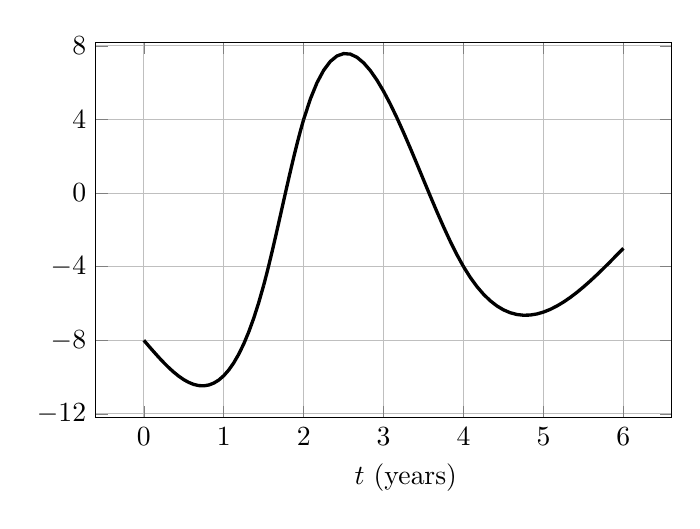
\begin{tikzpicture}
      \begin{axis}[grid=major, ytick={-12, -8, ..., 8}, ymax=8, ymin=-12,
        xlabel=$t$ (years), enlarge y limits=0.01,
        width=3.5in, height=2.5in, axis
          line style={shorten >=-8pt, shorten <=-8pt}, xlabel
          style={xshift=8pt}]
   %          \addplot[very thick][domain=0:1]{+3.0892857142857144*x^3+6.357142857142857e-61*x^2+-0.08928571428571429*x^1+-15*x^0};
			% \addplot[very thick][domain=1:2]{+-6.446428571428571*x^3+28.607142857142858*x^2+-28.696428571428573*x^1+-5.464285714285714*x^0};
			% \addplot[very thick][domain=2:4]{+2.3169642857142856*x^3+-23.973214285714285*x^2+76.46428571428571*x^1+-75.57142857142857*x^0};
			% \addplot[very thick][domain=4:6]{+-0.6383928571428571*x^3+11.491071428571429*x^2+-65.39285714285714*x^1+113.57142857142857*x^0};
            \addplot[very thick][domain=0:1.5]{+3.1384976525821595*x^3+2.4611267605633803e-60*x^2+-5.061619718309859*x^1+-8*x^0};
			\addplot[very thick][domain=1.5:2]{+-20.739436619718308*x^3+107.45070422535211*x^2+-166.23767605633802*x^1+72.58802816901408*x^0};
			\addplot[very thick][domain=2:4]{+3.819982394366197*x^3+-39.90580985915493*x^2+128.47535211267606*x^1+-123.88732394366197*x^0};
			\addplot[very thick][domain=4:6]{+-0.9889964788732394*x^3+17.801936619718308*x^2+-102.3556338028169*x^1+183.88732394366198*x^0};
      \end{axis}
    \end{tikzpicture}
  \end{tabular}

  We'd like to approximate the net change in the amount of oil in the SPR
  between $t = 0$ and $t = 6$.  As you learned in class, the idea is to
  partition the time interval into smaller intervals in which we can treat
  the rate as approximately constant. As a \emph{very crude} approximation,
  let's partition the interval $[0,6]$ into $3$ equal time intervals:
  $[0,2]$, $[2,4]$, $[4,6]$. 
  \begin{enumerate}
  \item
\begin{problem}[\vfill]
      At what rate was oil entering/leaving the SPR at $t = 0$?  (Give
      your answer with units, and be sure to say whether the oil was
      entering or leaving.)
    \end{problem}

    \begin{solution}
      Since $f(0) = - 8$, oil was leaving at a rate of 8 million barrels
      per year.
    \end{solution}

  \item
\begin{problem}[\vfill]
      If we \emph{assume}, for the purposes of approximation and simplicity, that oil
      entered/left the reserve at a \emph{constant} rate (namely, the rate
      you found in {{{{\#1}}(a)}}) between $t = 0$ and $t
      = 2$, how much oil entered/left in that time period?  (Give your
      answer with units, and be sure to say whether the oil entered or
      left the reserve.)
    \end{problem}

    \begin{solution} 
      We're assuming that oil left at a constant rate of $8$ million
      barrels per year for 2 years; in that case, (15 million
      barrels/year)(2 years) = 16 million barrels would have left the
      reserve.
    \end{solution}

  \item
    \begin{problem}[\vfill\newpage]
      At what rate was oil entering/leaving the reserve at $t = 2$?
    \end{problem}

    \begin{solution}
      Since $f(2) = 4$, oil was entering at a rate of 4 million barrels
      per year.
    \end{solution}

  \item
\begin{problem}[\vfill]
      If we assume that oil entered/left the reserve at this same rate
      between $t = 2$ and $t = 4$, how much oil entered/left in that time
      period?
    \end{problem}

    \begin{solution}
      Then, (4 million barrels/year)(2 years) = 8 million barrels
      would have entered.
    \end{solution}

  \item
    \begin{problem}[\stretch{0.5}]
      At what rate is oil entering/leaving the reserve at $t = 4$?      
    \end{problem}

    \begin{solution} 
      Since $f(4) = -4$, oil was leaving at a rate of 4 million barrels
      per year.
    \end{solution}

  \item
\begin{problem}[\stretch{0.5}]
      If we assume that oil entered/left the reserve at this same rate
      between $t = 4$ and $t = 6$, how much oil entered/left in that time
      period?
    \end{problem}

    \begin{solution}
      Then, (4 million barrels/year)(2 years) = 8 million barrels would
      have left.
    \end{solution}

  \item
\begin{problem}[\vfill]
      Use your answers to {{{{\#1}}(b)}},
      {{{{\#1}}(d)}}, and {{{{\#1}}(f)}} to
      estimate the net change in the amount of oil from $t = 0$ to $t =
      6$.  Based on this very crude approximation, was this a net gain or a
      net loss? 
    \end{problem}

    \begin{solution}
      We estimated that the reserve would lose 30 million barrels, have no
      net change, then lose another 10 million barrels, for a net
      change of $-16 + 8 - 8 = - 16$ million barrels.  This is a
      \fbox{net \emph{loss} of 16 million barrels}.
    \end{solution}

  \item
    \begin{problem}[\stretch{0.5}]
      Illustrate your answer to {{{{\#1}}(g)}} on the graph
      of $f$.  Did you do a right-hand or left-hand approximation? 
    \end{problem}

    \begin{solution} % Jason Bland
      The net change can be represented as a signed area of rectangles,
      with the green area contributing a positive net change and the red
      area contributing a negative net change:

      \begin{tabular}{c}
        {\small rate of change of amount of oil in the SPR} \\ 
        {\small (millions of barrels / year)} \\
        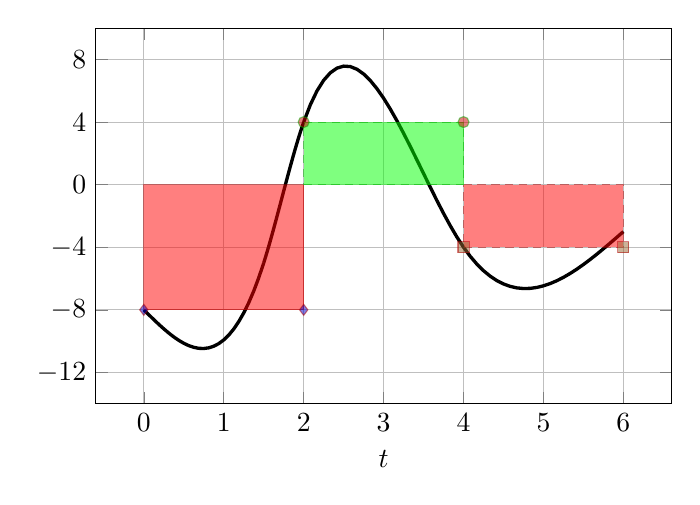
\begin{tikzpicture}
          \begin{axis}[grid=major, ytick={-12, -8, ..., 8}, ymax=8, ymin=-12,
          xlabel=$t$, enlargelimits=true,
            width=3.5in, height=2.5in]
            \addplot[very thick][domain=0:1.5]{+3.1384976525821595*x^3+2.4611267605633803e-60*x^2+-5.061619718309859*x^1+-8*x^0};
			\addplot[very thick][domain=1.5:2]{+-20.739436619718308*x^3+107.45070422535211*x^2+-166.23767605633802*x^1+72.58802816901408*x^0};
			\addplot[very thick][domain=2:4]{+3.819982394366197*x^3+-39.90580985915493*x^2+128.47535211267606*x^1+-123.88732394366197*x^0};
			\addplot[very thick][domain=4:6]{+-0.9889964788732394*x^3+17.801936619718308*x^2+-102.3556338028169*x^1+183.88732394366198*x^0};
            \addplot+[ybar interval, fill=red, opacity=0.5,
            draw=red!70!black] coordinates 
            {
              (0, -8)
              (2, -8)
            };        
            \addplot+[ybar interval, fill=green, opacity=0.5,
            draw=green!70!black] coordinates 
            {
              (2, 4)
              (4, 4)
            };        
            \addplot+[ybar interval, fill=red, opacity=0.5,
            draw=red!70!black] coordinates 
            {
              (4, -4)
              (6, -4)
            };        
          \end{axis}
        \end{tikzpicture}
      \end{tabular}

      This is a left hand approximation.
    \end{solution}

  \end{enumerate}

  \pspace{\newpage}

\item

\begin{grading}
8 points. 4 for each part.
\end{grading}


Maple syrup is being poured at a decreasing rate out of a tank.  By
  taking readings from the valve on the tank, we have the following
  information on the rate at which the syrup is leaving the tank.

  \begin{tabular}{l|c|c|c|c|c}
    $t$ (seconds)& $0$& 2& 4& 6& 8\\
    \hline
    rate (in cm$^3$/sec)& 10& 9& 7& 4& 2
  \end{tabular}

  \begin{enumerate}

  \item
\begin{problem}[\vfill]
      Find a good overestimate (also known as an \emph{upper bound}) for
      the amount of maple syrup that has been poured out between time $t =
      0$ and $t = 8$.
    \end{problem}

    \begin{solution} % Jason Bland
      Between times $t = 0$ and $t = 2$, the rate at which the syrup is
      leaving the tank stays between 9 and 10 cm$^3$/s.  A good
      overestimate would be to assume the rate is 10 cm$^3$/s throughout
      this time interval. In this case we would get
      \[ \text{amount of maple syrup poured out between $t = 0$ and $t =
        2$} \approx (10 \text{ cm$^3$/s})(2 \text{ s}) = 20 \text{ cm}^3.\]
      Similarly, we can make the following overestimates:
      \begin{align*}
        \text{amount poured out between $t = 2$ and $t = 4$} & \approx (9
        \text{ cm$^3$/s})(2 \text{ s}) = 18 \text{ cm}^3 \\
        \text{amount poured out between $t = 4$ and $t = 6$} & \approx (7
        \text{ cm$^3$/s})(2 \text{ s}) = 14 \text{ cm}^3 \\
        \text{amount poured out between $t = 6$ and $t = 8$} & \approx (4
        \text{ cm$^3$/s})(2 \text{ s}) = 8 \text{ cm}^3 
      \end{align*}
      Thus, between $t = 0$ and $t = 8$, we get the overestimate $20 + 18
      + 14 + 8 = \boxed{60 \text{ cm}^3}$ for the total amount of syrup
      poured out.
    \end{solution}

  \item
    \begin{problem}[\vfill]
      Find a good underestimate (or \emph{lower bound}) for this same
      amount.
    \end{problem}

    \begin{solution} % Jason Bland
      We use the same basic idea as in {{{{\#2}}(a)}}, but now
      instead of using the rate at the beginning of each sub-interval as
      our approximate rate, we use the rate at the \emph{end} of the
      sub-interval; this will give an underestimate because the syrup
      comes out more slowly as time goes on:
      \begin{align*}
        \text{amount poured out between $t = 0$ and $t = 2$} & \approx (9
        \text{ cm$^3$/s})(2 \text{ s}) = 18 \text{ cm}^3 \\
        \text{amount poured out between $t = 2$ and $t = 4$} & \approx (7
        \text{ cm$^3$/s})(2 \text{ s}) = 14 \text{ cm}^3 \\
        \text{amount poured out between $t = 4$ and $t = 6$} & \approx (4
        \text{ cm$^3$/s})(2 \text{ s}) = 8 \text{ cm}^3 \\
        \text{amount poured out between $t = 6$ and $t = 8$} & \approx (2
        \text{ cm$^3$/s})(2 \text{ s}) = 4 \text{ cm}^3 
      \end{align*}
      Therefore, the total amount poured out between $t = 0$ and $t = 8$
      is $\approx 18 + 14 + 8 + 4 = \boxed{44  \text{ cm}^3}$. 
    \end{solution}

  \end{enumerate}


 \item 

\begin{grading}
15 points. 5 for each part.
\end{grading}

In this problem, we are interested in the area between the graph of
  $\sin x$ and the $x$-axis for $x$ in the interval $\left[0,
    \frac{\pi}{2} \right]$.  (This is the shaded area in the graph below.) 

  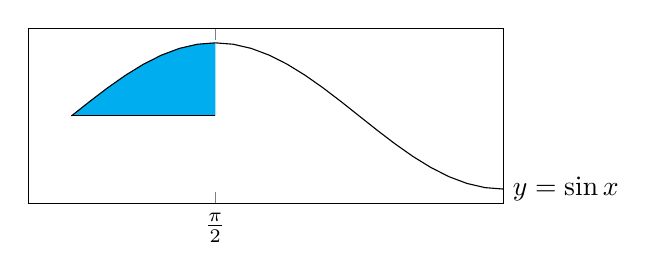
\begin{tikzpicture}
    \begin{axis}[cycle list=black, width=3in, height=1.5in, xmax=4.72,
      xtick=1.57, xticklabels={$\frac{\pi}{2}$}, ytick=\empty, clip=false]
      \addplot+[domain=0:pi/2, fill=cyan, draw=none] {sin(deg(x))} \closedcycle;
      \addplot+[domain=0:3*pi/2] {sin(deg(x))} node[right]{$y = \sin x$};
      \addplot+[domain=0:pi/2, thin] {0};
    \end{axis}
  \end{tikzpicture}

  \begin{enumerate}

  \item
\begin{problem}[\stretch{2}]
      Recall that we use the notation $L_3$ to mean the left-hand sum with
      three rectangles (of equal width) that estimates this area.  Find
      $L_3$; give an exact answer.  Draw a picture illustrating $L_3$.  Is
      $L_3$ an overestimate or underestimate for the area we're interested
      in?
    \end{problem}

    \begin{solution} % Jason Bland
      We can picture $L_3$ as the area in the green rectangles, which
      shows that it's an \fbox{underestimate}.
      \begin{center}
        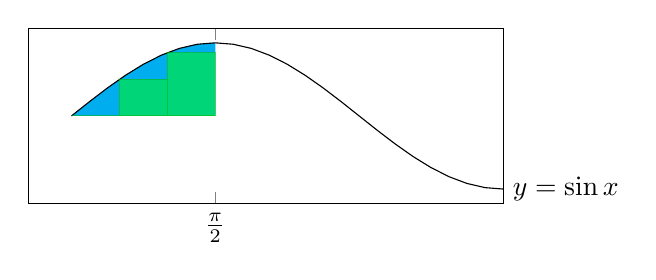
\begin{tikzpicture}
          \begin{axis}[cycle list=black, width=3in, height=1.5in, xmax=4.72,
            xtick=1.57, xticklabels={$\frac{\pi}{2}$}, ytick=\empty, clip=false]
            \addplot+[domain=0:pi/2, fill=cyan, draw=none] {sin(deg(x))} \closedcycle;
            \addplot+[domain=0:3*pi/2] {sin(deg(x))} node[right]{$y = \sin x$};
            \addplot+[ybar interval, fill=green, opacity=0.5,
            draw=green!70!black] coordinates 
            {
              (0, 0)
              (0.5236, 0.5)
              (1.0472, 0.866)
              (1.5708, 0.866)
            };        
          \end{axis}
        \end{tikzpicture}
      \end{center}
      (Note that the first rectangle has height 0.)

      Each of the rectangles has width $\frac{\pi}{6}$, so
      \begin{align*}
        L_3 &= \sin(0) \cdot \frac{\pi}{6} + \sin \left( \frac{\pi}{6}
        \right) \cdot \frac{\pi}{6} + \sin \left( \frac{2 \pi}{6} \right)
        \cdot \frac{\pi}{6} \\
        &= 0 + \frac{1}{2} \cdot \frac{\pi}{6} + \frac{\sqrt{3}}{2} \cdot
        \frac{\pi}{6} \\
        &= \boxed{\frac{\pi (1 + \sqrt{3})}{12}}
      \end{align*}
    \end{solution}

    \pspace{\newpage}

  \item
    \begin{problem}[\vfill]
      Repeat {{{{\#3}}(a)}} using a right-hand sum rather than
      a left-hand sum.
    \end{problem}

    \begin{solution} % Jason Bland
      This time we are interested in $R_3$, which is an \fbox{overestimate}:

      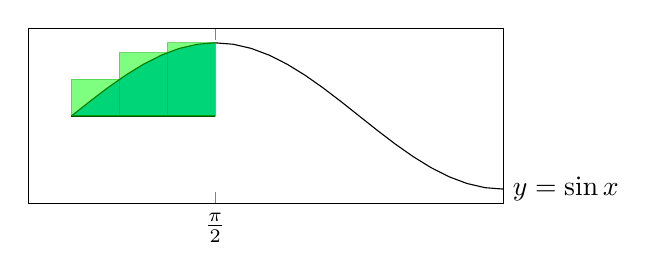
\begin{tikzpicture}
        \begin{axis}[cycle list=black, width=3in, height=1.5in, xmax=4.72,
          xtick=1.57, xticklabels={$\frac{\pi}{2}$}, ytick=\empty, clip=false]
          \addplot+[domain=0:pi/2, fill=cyan, draw=none] {sin(deg(x))} \closedcycle;
          \addplot+[domain=0:3*pi/2] {sin(deg(x))} node[right]{$y = \sin x$};
          \addplot+[domain=0:pi/2, thin] {0};
          \addplot+[ybar interval, fill=green, opacity=0.5, draw=green!70!black] coordinates
          {
            (0, 0.5)
            ({pi/6}, {sqrt(3)/2})
            ({pi/3}, 1)
            ({pi/2}, 0)
          };
        \end{axis}
      \end{tikzpicture}

      \begin{align*}
        R_3 &= \sin \left( \frac{\pi}{6} \right) \cdot \frac{\pi}{6} +
        \sin \left( \frac{2 \pi}{6} \right) \cdot \frac{\pi}{6} + \sin
        \left( \frac{3 \pi}{6} \right) \cdot \frac{\pi}{6} \\
        &= \frac{1}{2} \cdot \frac{\pi}{6} + \frac{\sqrt{3}}{2} \cdot
        \frac{\pi}{6} + 1 \cdot \frac{\pi}{6} \\
        &= \boxed{\frac{\pi (3 + \sqrt{3})}{12}}
      \end{align*}
    \end{solution}

  \item
    \begin{problem}[\vfill]
      Use the Riemann Sum\footnote{Left-hand sums and right-hand sums are
        both examples of ``Riemann sums.''  We'll talk more about what the
        term ``Riemann sum'' means in the coming days.} applet at
      \url{https://www.geogebra.org/m/sgxnjavg} to find $L_{50}$ and
      $R_{50}$.  (You can also use it to check your answers for $L_3$ and
      $R_3$.)  Based on these, what do you think the actual area we're
      looking for might be?

      To use the applet, type \texttt{sin(x)} in the box for $f(x)$,
      \texttt{0} in the box for $a$, and \texttt{pi/2} in the box for $b$;
      then click the ``Update'' button.  Use the slider to adjust the
      number of rectangles, and use the checkboxes to switch between the
      right-hand and left-hand sum.
    \end{problem}

    \begin{solution} 
      $L_{50}$ is 0.98421 and $R_{50}$ is 1.01563, which suggests the
      exact area might be 1.
    \end{solution}

  \end{enumerate}


  \pspace{\newpage}


\item 

\begin{grading}
15 points as follows: 5/5/5 (1 pt for each subpart of c)
\end{grading}

\note{This problem has two purposes.  The first is to give them a
    decreasing function, so that they don't jump to the conclusion that
    right-hand approximations are always overestimates.  The second is to
    get them to start thinking about notation and how we get the area of
    the $k$-th rectangle.}

  In this problem, we're interested in the area between the graph of
  $\dfrac{1}{x}$ and the $x$-axis for $x$ in the interval $[1, 3]$.
  \begin{enumerate}
  \item
\begin{problem}[\vfill]
      Find $R_4$, the right-hand sum with 4 rectangles that approximates
      this area; please give your answer as a fraction.  
    \end{problem}

    \begin{solution} % Jason Bland
      We're splitting an interval of width $3 - 1 = 2$ into 4
      sub-intervals, so each will have width $\frac{2}{4} = 0.5$.  Here's
      a picture of $R_4$:
      \begin{center}
        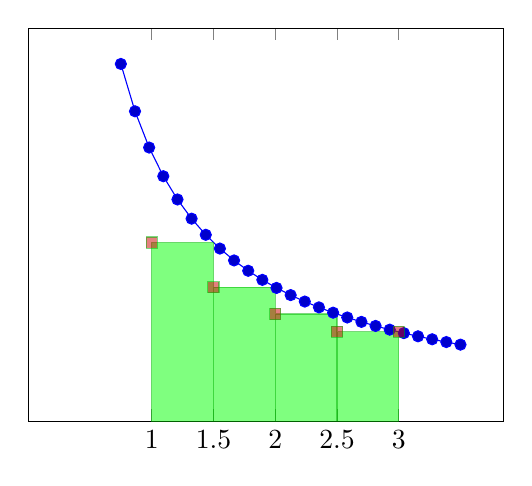
\begin{tikzpicture}
          \begin{axis}[width=3in, xmin=0, ymin=0, xtick={1, 1.5, 2, 2.5,
              3}, ytick=\empty] 
            \addplot+[domain=0.75:3.5] {1/x};
            \addplot+[ybar interval, fill=green, opacity=0.5,
            draw=green!70!black] coordinates 
            {
              (1, {1/1.5})
              (1.5, {1/2})
              (2, {1/2.5})
              (2.5, {1/3})
              (3, {1/3})
            };                    
          \end{axis}
        \end{tikzpicture}
      \end{center}
      From the picture, we can see that
      \[ R_4 = \frac{1}{1.5} \cdot 0.5 + \frac{1}{2} \cdot 0.5 +
      \frac{1}{2.5} \cdot 0.5 + \frac{1}{3} \cdot 0.5 =
      \boxed{\frac{19}{20}}.\]
    \end{solution}

  \item
    \begin{problem}[\vfill]
      Draw a picture illustrating how $R_4$ relates to the area we're
      looking for.  Is $R_4$ an overestimate or underestimate for the
      actual area? 
    \end{problem}

    \begin{solution}
      From the picture we drew in
      {{{{\#4}}(a)}}, we can see that $R_4$ is
      an \fbox{underestimate}. 
    \end{solution}

\pspace{\newpage}
    

  \item Use the Riemann Sum applet at \url{https://www.geogebra.org/m/sgxnjavg} to check your answers to the previous
    parts.

    To use the applet, type \texttt{1/x} in the box for $f(x)$,
      \texttt{1} in the box for $a$, and \texttt{3} in the box for $b$;
      then click the ``Update'' button.  Use the slider to adjust the
      number of rectangles, and use the checkboxes to switch between the
      right-hand and left-hand sum.

    As you can see in the applet (if you use it with 5 or fewer
    rectangles), it can be convenient to name the $x$-values where the
    rectangles' edges lie as $x_0, x_1, x_2$, and so on.  Suppose we now
    want to find $R_{10}$, the right-hand sum with 10 rectangles.
    \begin{enumerate}
    \item
      \begin{problem}[\vfill]
        How wide should each rectangle be?
      \end{problem}

      \begin{solution} 
        Since the entire interval $[1, 3]$ has width 2, each rectangle
        would have width $\frac{2}{10} = \boxed{0.2}$.
      \end{solution}

    \item
      \begin{problem}[\vfill]
        If we again labeled the $x$-values where the rectangles' edges lie
        as $x_0, x_1, x_2, \ldots, x_{10}$, what would $x_1$ be?  How
        about $x_4$?
      \end{problem}

      \begin{solution}
        To get from $x_0 = 1$ to $x_1$, we move to the right by one
        rectangle's width, so $x_1 = x_0 + 0.2 = 1.2$.

        To get from $x_0 = 1$ to $x_4$, we move to the right by 4
        rectangles' widths, so $x_4 = 1 + 4 (0.2) = 1.8$.
      \end{solution}

    \item
      \begin{problem}[\vfill]
        What is the area of the left-most rectangle?  (Please give your
        answer as a fraction.) 
      \end{problem}

      \begin{solution} % Jason Bland
        The width is $0.2$ while the height is $\frac{1}{x_1} =
        \frac{1}{1.2}$, so the area is $\frac{1}{1.2} \cdot 0.2 =
        \boxed{\frac{1}{6}}$.
      \end{solution}

    \item
      \begin{problem}[\vfill]
        What is the area of the 7th rectangle from the left?  (Please give
        your answer as a fraction.)

        \emph{Hint:} Since we're doing a right-hand approximation, you
        need to figure out at what $x$-value the right side of the 7th
        rectangle is.  
      \end{problem}

      \begin{solution} % Jason Bland        
        The 7th rectangle from the left lies between $x = x_6$ and $x =
        x_7$, so its height is $ \frac{1}{x_7} = \frac{1}{1 + 7(0.2)}$.
        Therefore, its area is $\frac{1}{1 + 7 (0.2)} \cdot 0.2 =
        \frac{1}{12}$.
      \end{solution}

    \item
      \begin{problem}[\vfill]
        Use the applet to find $R_{10}$. 
      \end{problem}

      \begin{solution} 
        $1.0349$.
      \end{solution}

    \end{enumerate}

  \end{enumerate}

\pspace{\newpage}


\item 

\begin{grading}
5 points.
\end{grading}

\textbf{Reflect Back.} % (basically 22.2.1) 
  \begin{problem}[\stretch{2}]
    Below are the graphs of the velocities of three runners on the
    interval $[0, 5]$.
    Who has traveled the greatest distance in this 5-minute time interval?
    Who has traveled the smallest distance in the time interval?  Explain
    how you know.

    
\includegraphics{images/go22p02.pdf}

  \end{problem}

  \begin{solution} % Jason Bland
    Runner A was consistently the fastest, and Runner C was consistently
    the slowest. Since all 3 runners ran for the same amount of time, A
    must have traveled the most distance while C traveled the least.
  \end{solution}

\end{enumerate}

\psreflection{
Optional reading for next class is \S 22.2, 22.3 in Gottlieb.
}

\end{document}